\section{Experimental Study}\label{sec:expr}
We implemented our approach in a tool called \tool written in C++ interfacing MINISAT 2.2 \cite{MINISAT}.
It's available at xxx.
In this section, we present the experimental results of \tool.
There are 3 industrial benchmarks, consists of 72 industrial satisfiable formulae and 86 random benchmark, consisted 6606 generated satisfiable formulae. Each formula in an industrial benchmark is selected from verification of the same application, each formula in a random benchmark are generated from the same unsatisfiable formula. Formulae in the same benchmark share some common features, such as the number of variables and clauses, the structure of the formula and so on.

The experiments were conducted on a cluster of IBM iDataPlex 2.83 GHz, each industrial formula was running with a timeout of 1800s and memory limit of 4GB. Each random formula was running with a timeout of 100s and memory limit of 256 MB. Our experiments benefit from the small scale of generated formulae, which allow us to run more formulae at the same time.

For industrial formulae, both \tool and \minibones are able to solve 34 formulae out of 72. For generated formulae, both \tool and \minibones are able to solve the total 6606 formulae under time and memory limits.
Experiments show that for \textit{mrpp} benchmark, \minibones solved 4\% times faster, and for $\textit{manthey}$ benchmark, \tool reduces 38\% solving time. \tool reduces 2183 seconds of solving time of industrial formulae, saving 21\% solving time in total.

When we take a close look at the formulae that are accelerated by \tool from industrial benchmark, we found that the adjacent structure of these formulae shared some common features. Experiments show that different formula has different structures, formulae from the same benchmark often have similar structures. Compared with the ball-like structure for formulae in $\textit{mrpp}$, formulae in $\textit{manthey}$ benchmark have more star-like structures. There are two formulae in $\textit{mrpp}$ that have a pipe-like structure, where there are several branches near the main root-like core, \tool performs better on this two formula.
\subsection{Benchmark Setup}
We select 72 industrial formulae from SAT competitions, 34 are them are solved by both \tool and \minibones. We also select 100 crafted formulae from SAT competitions, none of them are solved within time and memory limits. In order to test the scalability of \tool, we generate 6606 satisfiable formulae from unsatisfiable formulae. The reason we don't choose random satisfiable formulae is because they have different community structures. Generated formulae from the same unsatisfiable formula share similar community structure from nature. We would like to explore the relationship between features of structures of the formula and the performance of \tool. Another reason is that, unlike other random formula that requires more than 500 seconds solving time, the solving time of generated formula range from 1 seconds to 100 seconds, which saved lots of solving time and make our experiments more practicable.

There are 3 benchmarks among industrial formulae, which are $\textit{mrpp}$, $\textit{manthey}$ and $\textit{dimacs}$. The comparison between \tool and \minibones are analyzed in different benchmarks.
For generated formulae, they are grouped into 100 benchmark since there are 100 different formulae that generate them.

We separate formulae into different benchmarks to study the effects of different adjacent structures on the performance of \tool. Adjacent structures are presented as adjacent graph of a formula. The nodes in the graph stands for variables, if two variables shared the same clause, there is an edge between them. In the graph, the more adjacent variables a variable has, the more center the variable located. In the middle of an adjacent graph, there is a ball-like core formed by variables that has multiple neighbours, if a variable has less neighbours, it will locate apart from the core, the less neighbours a variable has, the farer it located to the core.

\subsection{Experimental Results on Industrial Formulae}
The general result of industrial formulae
SAT solving time and SAT calls of different benchmark, with different proportion.
A line graph that describes SAT solving time comparison.

Show the density of $\BLap(\Phi)$ and the original formula, show them in line graph, they should be always higher.

Analysis the relationship between adjacent structure and the accelerating performance, give two structures as example. The ball-like one are hard for both \tool and \minibones. But \tool performs better on branch-like ones, thanks to the remove of non-backbone ahead and the high possible of backbone, all increase the chance that we hit one of the variables in the branch, and SAT solving will be rather fast. Since variables are less connected with each other and less conflicts will arise.


SAT solving time and SAT calls of different benchmark, only with Algorithm 1.
The same table and analysis for Algorithm 2. a table with 1, 2, 1+2.
A general comparison result about Algorithm 1 and Algorithm 2.
The results show that for formulae in $\textit{manthey}$, the combination is the best. The contribution is almost the same.
For $\textit{mrpp}$, the combination is not the best solution, this explains why our algorithm performs poorly on this benchmark, one step of the computing doesn't behaves well. It's because that the formula in this benchmark are hard to test whether a literal is a backbone,(seen the gap between the first model solving time and the total solving time). The reason for this is because the variables here shared a very tight relations, it will causes lots of conflicts by mis-assignement any of them.


\begin{table}[t]
\centering
\begin{tabular}{ccccc}
\toprule
 &Total  Time (s) & SAT Calls&Average Time (s)\\
\midrule
\tool&26663  &272089&0.9890  \\
cb100&30295  &239112&1.0174  \\
\bottomrule
\end{tabular}
\caption{Experimental results for 138 industrial formulae}
\label{tab:ind}
\end{table}

Table \ref{tab:ind} shows the overview of experimental results on industrial formulae.
Among all the 388 industrial formulae, there are 138 formulae that both \tool and \textit{cb100} were able to compute backbone within 1800s.
Although, the number of SAT calls used by \tool is greater than \textit{cb100}, \tool reduces by 12\% of the total running time and by 11\% of the average running time for each SAT call.

Figure \ref{fig:ind-time} provides the details of experimental results on industrial formulae, including the running time of the SAT solver for generating the first model and total running time for each formula.
The red dotted line represents for the time used by the SAT solver for computing the first model, which indicates the hardness of the formula.
Lines with crosses represents for the running time of \tool, and lines with boxes represents for the running time of \textit{cb100}. There is a correlation between the hardness of formulae the performance of \tool comparing to \textit{cb100}.
For most of hard formulae, \tool outperforms \textit{cb100} in terms of total running time and average time of each SAT solver call. This demonstrates that \tool is more feasible for computing backbone of hard formulae.

%\textit{cb100} highly rely on the quality of model returned by SAT solver, it performances better when SAT solver gave it a suitable model. For most of the formulae that need less than 1 second to compute a first model, both \tool and \textit{cb100} were able to compute backbone very quickly with barely difference.

Table \ref{tab:ind} and Figure \ref{fig:ind-time} demonstrate that \tool outperforms \textit{cb100} on industrial formulae.


\begin{figure}
    \centering
    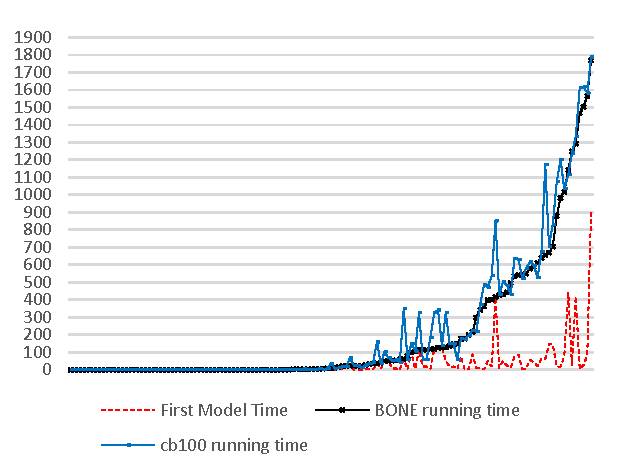
\includegraphics[scale=0.8]{ind2.pdf}
   \caption{Experimental results on industrial formulae}
   \label{fig:ind-time}
\end{figure}



\section{Results for Generated Formulae}
How many solving time saved in total, what proportion.
Show the total solving time and SAT calls of selected 3 benchmark, accelerating 1, the same 1, decline 1.
Show the statistic results of different benchmarks, how many accelerating, more than how large proportion, how many the same, how many decline, at how large proportion

Explain the relation between adjacent structure and performance.
3 pictures

Based on this observation, we divide 6606 random formulae into three groups according to their community structures.
The \emph{simple group} contains 371 formulae whose community structures are divergent,
the \emph{hard group} contains 337 formulae whose community structures are focusing,
and the \emph{medium} group contains 5898 formulae between divergent and focusing.


Table \ref{tab:mcs-graph} shows the experiments results on these three groups. \textit{cb100} performs better than \tool on the simple group, as \textit{cb100} tries to find a backbone literal by complementing models as soon as possible, which are the vertexes far from the center.
\tool outperforms \textit{cb100} for both medium group and hard group.
\tool reduces by 8\% for medium group and by 40\% for hard group of the total running time.

The experimental results show that \tool performs better than \textit{cb100} on hard random formulae and is comparable to \textit{cb100} on simple formulae.

NOTE: draw the community structure of the unsatisfiable formula
For formulae generated from an unsatisfiable formula with a very sharp community structure, that is there is exactly one obvious edge that sperate away from the core of variables, \tool performs quite well, almost needs less than 5 seconds to compute backbone.
For formulae generated from an unsatisfiable formula with a ball-like structure, both \tool and \minibones need almost more than 20 seconds to solve. This indicates that ball-like structure are hard to complex backbone. If we compare the solving time of first model between type I and type II, we can find that it's more changeling for MINISAT to solve type II, because there is no short-cut to find a good assignment quickly.
For the rest of formula, a core with multiple branches around the core, \tool performs better than \minibones on most of the generated formulae.




